\documentclass[conference]{IEEEtran}
% Based on the supplied conference_101719.tex IEEE conference template.
% No margins, column widths, font sizes, or line spacing are overridden.
\usepackage[T1]{fontenc}
\usepackage{cite}
\usepackage{amsmath,amssymb,amsfonts}
\usepackage{graphicx}
\usepackage{textcomp}
\usepackage{xcolor}
\usepackage{booktabs}
\usepackage{url}
\usepackage{balance}
\graphicspath{{figures/}}
\def\BibTeX{{\rm B\kern-.05em{\sc i\kern-.025em b}\kern-.08em
    T\kern-.1667em\lower.7ex\hbox{E}\kern-.125emX}}

\begin{document}

\title{Context-Aware Anomaly Detection and Health Monitoring of Turbofan Engines}
\author{\IEEEauthorblockN{Selvakumar Sadurshan}
\IEEEauthorblockA{sadushansadu33@gmail.com}}
% Add the author's verified department, institution, city, and country here.
% No affiliation, funding, or additional author has been assumed.
\maketitle

\begin{abstract}
Operating-condition changes and engine-specific sensor offsets complicate the interpretation of degradation in multivariate engine data. This paper presents an implemented anomaly detection and health monitoring component that combines operating-mode normalization, a commissioned healthy sensor reference, four complementary anomaly detectors, and an interpretable health trajectory. Isolation Forest, shrinkage covariance distance, a long short-term memory autoencoder, and a residual rule contribute equally to a frozen anomaly score. A separate residual-based health index provides continuous condition tracking and five health states. Evaluation uses all four NASA turbofan degradation subsets with shared, disjoint engine roles for fitting, calibration, development selection, and retrospective confirmation. Saved predictions were independently checked against the original test labels. On previously inspected official test trajectories, the four-detector system achieves a receiver operating characteristic area of 0.9952, precision of 0.8999, and recall of 0.6321 at its calibrated threshold. It detects critical-condition observations in 131 of 159 eligible engines, with 181 false alerts across 49,232 healthy-proxy cycles. The recomputed health index has a pooled remaining-life rank correlation of 0.4601 and a monotonicity pass fraction of 0.9477. The results demonstrate an auditable monitoring implementation while identifying threshold sensitivity, subset variation, and incomplete fault-label validation as limits. All detection labels are remaining-life condition proxies, and benchmark reuse precludes a blind generalization claim.
\end{abstract}

\begin{IEEEkeywords}
anomaly detection, condition monitoring, turbofan engines, health index, operating context, explainable machine learning
\end{IEEEkeywords}

\section{Introduction}
An engine monitoring system must distinguish a change in operating conditions from a change in equipment condition. A sensor reading can depart from its previous level because the operating regime changed, because an engine has a persistent individual offset, or because deterioration is developing. A useful monitoring output therefore needs an expected reference, evidence of deviation, a temporal interpretation, and a clear account of the observations for which a decision is available.

The Commercial Modular Aero-Propulsion System Simulation (C-MAPSS) benchmark provides multivariate turbofan trajectories with progressive degradation and operating-condition variation~\cite{saxena2008,nasaData}. Its life labels support reproducible condition-proxy evaluation, but do not by themselves identify the onset or physical cause of every abnormal sensor event. Treating all low-life observations as confirmed faults would overstate the available supervision. Likewise, reporting accuracy without the healthy-to-critical class distribution can obscure missed critical observations.

This work studies the implemented Anomaly and Health Monitoring component of an aircraft monitoring application. The component converts sensor histories into anomaly evidence, health trajectories, health states, explanations, and confidence indicators. Its scope ends at these monitoring outputs; remaining-life regression, maintenance scheduling, and supervisory action optimization are outside this study.

The contribution is an auditable integration and evaluation of existing methods, rather than a new isolation, covariance, or recurrent-learning algorithm. Specifically, the component provides: (1) a shared engine partition and frozen preprocessing references that separate model fitting from subsequent scoring; (2) a context-conditioned sensor reference with causal commissioning, followed by four-detector score fusion and a separate continuous health index; and (3) an evaluation that reports coverage, confusion counts, engine events, clustered uncertainty, health trajectories, and explanation fidelity together. A fixed linear sensor baseline provides a practical comparison and exposes the limits of assuming that additional detectors necessarily improve classification.

\section{Related Work}
Isolation Forest identifies observations that are readily isolated by random partitions~\cite{liu2008}. Its ranking is useful when deviations differ from the reference population, but it does not explicitly model sensor covariance or temporal reconstruction. Ledoit and Wolf~\cite{ledoit2004} provide a shrinkage covariance estimator that supports a numerically stable multivariate distance. These methods motivate complementary distributional views of residual behavior.

Malhotra \emph{et al.}~\cite{malhotra2016} reconstruct normal multivariate sequences with a long short-term memory (LSTM) encoder--decoder and use reconstruction error for anomaly evidence. The present component applies this established approach to causal residual windows, alongside distributional detectors and a transparent residual rule. The detectors are combined at the score level; the contribution does not include a new recurrent architecture.

Random forests~\cite{breiman2001}, XGBoost~\cite{chen2016}, and LightGBM~\cite{ke2017} provide established regression models for the expected sensor response. Here they operate with a dense neural regressor as an ensemble reference conditioned on operating settings and observed cycle position. This statistical reference is called a digital twin in the implementation, but no thermodynamic simulator or identified physical damage model is claimed.

SHapley Additive exPlanations (SHAP) assigns contributions to a model prediction~\cite{lundberg2017}. The implementation explains the healthy-reference prediction and separately ranks observed residuals. These are different explanatory objects: an attribution of the reference prediction is not an attribution of the entire fused anomaly decision. Evaluation methodology also matters. Kim \emph{et al.}~\cite{kim2022} show that point adjustment can inflate time-series detection results. Accordingly, this study retains observed cycle decisions and reports engine-level event measures separately, without filling an anomalous interval after a single successful detection.

\section{Monitoring Architecture and Problem Definition}
For engine $i$ at observed cycle $t$, let $\mathbf{u}_{i,t}\in\mathbb{R}^{3}$ denote operating settings and $\mathbf{x}_{i,t}\in\mathbb{R}^{p}$ the sensor vector. The evaluated bundle retains $p=21$ sensor channels. The monitoring task produces a continuous anomaly score $S_{i,t}\in[0,1]$, an alert classification, a health index $H_{i,t}\in[0,100]$, and associated evidence. Decisions use available observations and persisted model references. Remaining useful life (RUL) is used offline to identify training regions and evaluate condition proxies; it is not a serving-time predictor input.

Fig.~\ref{fig:architecture} shows the data flow. Cleaning, operating-mode discovery, and scaling precede the healthy reference. Residuals then feed two parallel branches: anomaly scoring and continuous health tracking. Explanation and confidence services attach evidence to the monitoring outputs. Learned references, thresholds, and the training-partition identity are persisted with the bundle.

\begin{figure*}[t]
\centering
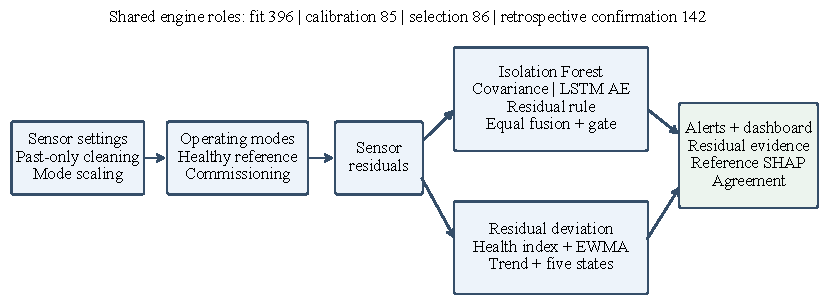
\includegraphics[width=\textwidth]{architecture.pdf}
\caption{Architecture of the evaluated anomaly and health monitoring component. Commissioning uses only prior observations. The health branch and anomaly branch share the monitoring residuals but have separate transformations and thresholds.}
\label{fig:architecture}
\end{figure*}

\subsection{Past-Only Preprocessing and Operating Context}
Rows are identified by engine and cycle, with distinct identities across subsets and train/test populations. Missing observations are repaired using earlier readings within the same engine and then frozen medians from fitting engines. No backward filling or inference-batch median fitting is used. Duplicate identities and missing learned references are treated as invalid inputs.

A persisted $k$-means model assigns operating modes from the three settings. The pooled fitted model contains six modes. Sensor and operating-setting scaling uses frozen mode-specific references; for a sensor,
\begin{equation}
\widetilde{x}_{i,t,j}=\frac{x_{i,t,j}-\mu_{k(i,t),j}}{\sigma_{k(i,t),j}},
\label{eq:scaling}
\end{equation}
where $\mu_{k,j}$ and $\sigma_{k,j}$ are the saved mean and scale of sensor $j$ in mode $k$. Unknown-mode handling uses persisted references per row, without fitting the evaluation population. A transition marker covers the mode-change cycle and the next three observed rows of the engine.

\subsection{Healthy Sensor Reference and Commissioning}
Each reference regressor uses mode-scaled operating settings, cycle $t$, fixed normalized age $\min(t/300,1)$, and six mode indicators. The 11-dimensional design excludes the current sensor targets, RUL, and eventual trajectory length. The four reference regressors are random forest, XGBoost, LightGBM, and a dense neural network. Their expected sensor vectors are combined with normalized inverse validation root mean squared error weights. The saved weights are 0.2511, 0.2391, 0.2503, and 0.2594, respectively.

Individual offsets are estimated from the first 30 observed cycles. At cycle $t$, the offset averages commissioning residuals strictly before $t$ and remains fixed after commissioning. With $f_m$ denoting reference model $m$ and $b^{(m)}_{i,t,j}$ its causal offset, the monitoring reference and residual are
\begin{align}
\widehat{x}^{\mathrm{ref}}_{i,t,j}
 &=\sum_{m=1}^{4}w_m\bigl(f_{m,j}(\mathbf{u}_{i,t},t,k)+b^{(m)}_{i,t,j}\bigr),\\
r_{i,t,j}&=\widetilde{x}_{i,t,j}-\widehat{x}^{\mathrm{ref}}_{i,t,j}.
\label{eq:residual}
\end{align}
This experiment uses the frozen context reference; optional adaptive sensor-forecast paths are excluded from the monitoring residuals. Alert evaluation begins only after a complete 30-cycle commissioning prefix. This requirement reduces coverage for short trajectories and is reported explicitly.

\section{Anomaly Detection and Health Estimation}
\subsection{Four Complementary Residual Detectors}
All four detectors receive the raw residuals of the mode-standardized sensor channels, rather than the separately available robust residual $z$ scores. Consequently, the constant 3 in the residual rule below is a residual-domain trigger, not a universal three-standard-deviation test.

Isolation Forest uses 200 trees, automatic subsampling, and random seed 42. Its negated decision function is mapped through a persisted empirical reference distribution. The covariance detector computes a trailing five-cycle residual mean and a squared Mahalanobis distance
\begin{equation}
D^2_{i,t}=(\overline{\mathbf{r}}_{i,t}-\boldsymbol{\mu})^{\!T}
\widehat{\boldsymbol{\Sigma}}^{-1}
(\overline{\mathbf{r}}_{i,t}-\boldsymbol{\mu}),
\end{equation}
using Ledoit--Wolf covariance shrinkage. Its bounded score is $s_{\mathrm{M}}=D^2/(D^2+q_{0.99})$, where $q_{0.99}$ is the saved healthy-reference distance percentile. Trailing covariance windows reset at observed cycle gaps.

The LSTM autoencoder receives 30-cycle windows. Its encoder has 64 and 32 units; the decoder has 32 and 64 units, with a time-distributed linear output. Dropout is 0.1. Training uses Adam with learning rate 0.001, batch size 128, at most 40 epochs, a 0.15 validation fraction within fitting windows, and early-stopping patience of six epochs. Mean squared reconstruction error over cycles and channels is converted to an empirical reference percentile. Inference windows end at the current observation, with first-reading padding at the start of a trajectory. The neural validation split is not an independent engine-level performance estimate.

The residual rule is
\begin{equation}
u_{i,t}=\frac{1}{p}\sum_{j=1}^{p}|r_{i,t,j}|+
0.5\sum_{j=1}^{p}\mathbb{I}(|r_{i,t,j}|>3),
\end{equation}
where $\mathbb{I}$ is the indicator function. Its score is the empirical percentile of $u_{i,t}$ under the stored healthy reference. Empirical percentile scores express position relative to a reference distribution; they are not calibrated fault probabilities.

\subsection{Score Fusion and Operational Gate}
The evaluated model fixes all detector weights to 0.25 before official-test evaluation:
\begin{equation}
S_{i,t}=\tfrac14(s_{\mathrm{IF}}+s_{\mathrm{M}}+s_{\mathrm{AE}}+s_{\mathrm{R}}).
\end{equation}
A score must be finite and available from every enabled detector. The calibrated threshold is not reused if one detector is absent. The fusion cutoff is the 99th percentile of fused scores on healthy calibration-role rows with RUL at least 125 and cycle greater than 30. Its persisted value is $\tau=0.90851712540986$; the alert condition is $S_{i,t}>\tau$ after readiness.

Consecutive above-threshold observations define persistence, with a reset at a cycle gap. During the context-transition marker, a flagged observation with fewer than three consecutive flags is classified as operational. Other ready flags are classified as fault alerts. Thus, three-cycle persistence is a transition-specific suppression rule, not a universal waiting period. Severity uses the relative threshold headroom $(S-\tau)/(1-\tau)$, with frozen medium, high, and critical boundaries of 0.41690, 0.67571, and 0.87042 fitted to fault-category rows from fitting engines. The word ``fault'' here names the software output category; the evaluation labels remain condition proxies.

\subsection{Continuous Health Index and States}
Health tracking uses a separate reference derived from healthy fitting-engine residuals. For the evaluated equal-channel policy, define
\begin{align}
d_{i,t}&=\frac{1}{p}\sum_j|r_{i,t,j}|,\\
h^{\mathrm{raw}}_{i,t}&=100\exp\!\left[-\lambda\max\left(\frac{d_{i,t}}{d_0}-1,0\right)\right],\\
H_{i,t}&=\alpha h^{\mathrm{raw}}_{i,t}+(1-\alpha)H_{i,t-1}.
\label{eq:health}
\end{align}
The saved healthy deviation reference is $d_0=0.3237016428571428$, based on 27,698 fitting-role rows. The active parameters are $\lambda=0.25$ and $\alpha=0.2$, with the first raw value initializing the exponentially weighted moving average (EWMA).

A separate health score adds half the three-cycle projection of the trailing 20-observation health slope and clips the result to $[0,100]$. Persisted state boundaries are 80, 60, 38, and 20 for Healthy, Degrading, Warning, Critical, and Failure Risk. These are operational categories, not probabilities of failure. Health-index evaluation uses $H$, without an additional evaluation-time smoothing pass.

\subsection{Explanations and Confidence Indicators}
An explanation combines the largest residuals, their temporal patterns, severity information, and a quantitative health decomposition. Grouped local SHAP explains operating-context and cycle-position contributions to the reference prediction, with the commissioning offset represented separately. The monitored residual remains the difference between the observed sensor and this explained reference. Sensor-to-subsystem rules provide diagnostic hypotheses; they do not establish physical causation.

The confidence indicator combines twin agreement, detector agreement, and data quality with weights 0.45, 0.35, and 0.20. It is an engineering support score. The experiment does not establish probability calibration, coverage guarantees, or expert-validated root-cause accuracy. Operator feedback can alter thresholds through a separate explicit workflow; automatic feedback updates are disabled during frozen scoring and offline refitting.

\section{Experimental Protocol}
\subsection{Data, Partitions, and Condition Labels}
Table~\ref{tab:data} gives counts independently reconstructed from the local NASA files. FD001 and FD003 have one operating condition; FD002 and FD004 have six. FD001 and FD002 contain one simulated fault mode; FD003 and FD004 contain two~\cite{nasaData}. Training trajectories end at failure. Official test trajectories are truncated, with supplied terminal RUL labels. For a test engine ending at cycle $T_i$, the evaluation reconstructs $\mathrm{RUL}_{i,t}=T_i-t+\mathrm{RUL}_{i,T_i}$.

\begin{table}[t]
\caption{C-MAPSS Data Used in This Study}
\label{tab:data}
\centering
\begin{tabular}{lrrrr}
\toprule
Subset & Train eng. & Train rows & Test eng. & Test rows\\
\midrule
FD001 & 100 & 20,631 & 100 & 13,096\\
FD002 & 260 & 53,759 & 259 & 33,991\\
FD003 & 100 & 24,720 & 100 & 16,596\\
FD004 & 249 & 61,249 & 248 & 41,214\\
\midrule
Total & 709 & 160,359 & 707 & 104,897\\
\bottomrule
\end{tabular}
\end{table}

One persisted plan separates the 709 training engines into 396 fitting, 85 healthy calibration, 86 development-selection, and 142 retrospective-confirmation engines. Learned preprocessing, operating context, reference models, and health references use the fitting role. Reference validation and ensemble weighting use selection engines; fused-cutoff calibration uses calibration engines. Confirmation engines and official test engines are excluded from these current fitting and selection operations. The four-detector anomaly experiment reuses the frozen sensor reference rather than refitting it.

Offline reference fitting selects RUL at least 130 within the initial 30\% of each fitting trajectory, while retaining at least the first ten rows per engine. Isolation Forest, autoencoder, and rule-reference selection use the early 30\% and RUL criterion; covariance fitting uses healthy post-commissioning rows. These complete-trajectory rules define offline reference populations only. At inference, fixed models, past observations, and commissioning offsets determine scores without RUL or future trajectory length.

Binary evaluation labels a row healthy when RUL is at least 125 and critical when RUL is at most 30. Intermediate RUL values 31--124 are excluded from binary metrics and retained in continuous trajectory and event analyses. These bands evaluate separation of distant condition states. They do not measure fault-onset classification, all-condition accuracy, or RUL prediction error.

\subsection{Coverage, Baseline, and Metrics}
The official input contains 104,897 rows from 707 engines. Commissioning excludes 21,109 rows and leaves 83,788 ready rows from 690 engines; 17 engines have no ready decision. Binary evaluation further excludes 31,982 intermediate rows, leaving 51,806 rows: 49,232 healthy and 2,574 critical. Coverage must accompany performance because excluded cycles and engines can affect operational usefulness.

The fixed sensor baseline is a previously measured logistic regression using nine current mode-standardized sensor channels: 2, 3, 4, 7, 11, 12, 15, 20, and 21. It uses L2 regularization with $C=1$, balanced class weights, and cutoff 0.5, and is fitted on healthy/critical rows from fitting engines. It shares the frozen preprocessing, commissioning coverage, and context gate. Its sensor list was developed on previously inspected data. This supervised proxy-label baseline differs from healthy-reference anomaly fitting, so the comparison is a practical reference rather than a controlled comparison of identical learning objectives.

Cycle-level metrics are precision, critical recall, F1, healthy-cycle false-alert rate, receiver operating characteristic area (ROC AUC), and average precision (AP). For example, $\mathrm{F1}=2\mathrm{TP}/(2\mathrm{TP}+\mathrm{FP}+\mathrm{FN})$ and $\mathrm{FAR}=\mathrm{FP}/(\mathrm{FP}+\mathrm{TN})$, where TP, FP, FN, and TN are true positives, false positives, false negatives, and true negatives. ROC AUC and AP use continuous scores; confusion metrics use the context-gated alert category. No point adjustment is applied.

Engine measures include detection of at least one critical observation among engines reaching the critical band, healthy engines with false alerts, and contiguous false-alert episodes. Confidence intervals resample whole engines with replacement, preserving all observations of each sampled engine, using 300 percentile-bootstrap replicates and seed 20261011. These intervals capture engine-sampling variation, not model-selection or benchmark-reuse uncertainty.

For health, pooled Spearman correlation relates health to RUL. The reported monotonicity measure is the fraction of engines for which at most 15\% of successive late-phase health changes exceed one point upward. Late phase is the last 70\% of the observed trajectory, with at least five observations required. This is a defined tolerance-based measure, not strict mathematical monotonicity. Early-to-late health change uses medians over $\min(20,\lfloor n_i/5\rfloor)$ observations at each end, subject to a minimum window of one. Median within-engine correlation is reported for eligible trajectories reaching the critical band.

\subsection{Evaluation Status and Reproducibility}
The official benchmark and training fleet were inspected during earlier development. Repartitioning and removing current leakage paths do not make these data blind. All reported generalization results therefore have retrospective benchmark status. The equal detector weights were fixed before this four-detector evaluation; official results did not determine its activation. No additional threshold selection is performed on the official labels for this paper.

The accompanying evidence script reads saved predictions, independently reconstructs original test labels, checks engine/cycle alignment, reconstructs fused scores, and recomputes confusion metrics, intervals, health trajectories, and figures. Health uses the same official residual input as the four-detector experiment and the current frozen health reference. A slightly different older saved health summary is retained for audit only, rather than substituted for this recomputation. The script records source-file hashes and the shared training-plan identity. It does not retrain the models or modify production outputs. Analysis uses Python with NumPy 1.26.4, pandas 2.2.3, scikit-learn 1.5.2, SciPy 1.14.1, and Matplotlib 3.9.4. No training-throughput or deployment-latency result is claimed.

\section{Results}
\subsection{Cycle-Level Detection and Baseline Comparison}
Table~\ref{tab:comparison} reports the actual operating point. The four-detector system yields 1,627 TP, 181 FP, 947 FN, and 49,051 TN. Its accuracy of 97.82\% exceeds the always-healthy accuracy of 95.03\%, but the critical-cycle recall is only 63.21\%. F1 and confusion counts are therefore more informative than accuracy alone. The 95\% whole-engine bootstrap intervals are [0.8230, 0.9593] for precision, [0.5734, 0.6948] for recall, [0.6962, 0.7864] for F1, and [0.00138, 0.00655] for healthy-cycle false-alert rate.

\begin{table}[t]
\caption{Retrospective Comparison on the Same Binary Condition Rows}
\label{tab:comparison}
\centering
\begin{tabular}{lrr}
\toprule
Metric & Linear baseline & Four detectors\\
\midrule
Accuracy (\%) & 98.99 & 97.82\\
Precision & 0.9045 & 0.8999\\
Critical recall & 0.8908 & 0.6321\\
F1 & 0.8976 & 0.7426\\
Healthy false alerts & 242 & 181\\
Missed critical rows & 281 & 947\\
Healthy-cycle FAR (\%) & 0.4916 & 0.3676\\
\bottomrule
\end{tabular}
\end{table}

The four-detector system reduces healthy false-alert rows relative to the fixed linear baseline while missing substantially more critical rows. It does not improve F1 or recall. Its ROC AUC of 0.9952 and AP of 0.8860 describe ranking over the two condition bands and must be interpreted separately from the selected cutoff. A high AUC can coexist with a conservative operating point and limited recall.

Fig.~\ref{fig:detection} plots precision--recall curves from the saved scores and marks the deployed gated operating point. Individual detector curves are diagnostic rankings on the same binary observations, not newly calibrated standalone deployments or retrained ablations. Their different score distributions, including covariance's rational transformation and the other detectors' empirical percentiles, make equal weighting simple to inspect but do not guarantee an optimal operating point.

\begin{figure*}[t]
\centering
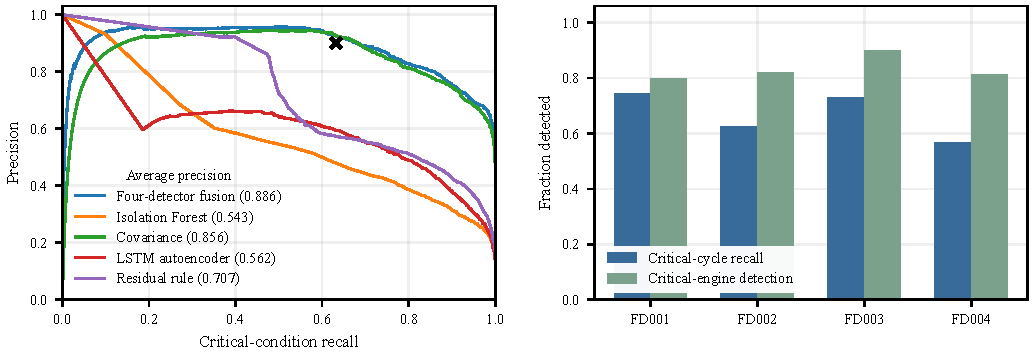
\includegraphics[width=\textwidth]{detection_results.pdf}
\caption{Retrospective detection evidence. Left: precision--recall rankings for the fused and individual saved scores; AP is shown in parentheses. The cross marks the deployed context-gated fused decision. Right: critical-cycle recall and the fraction of critical-reaching engines with at least one critical alert. No interval filling or test-label threshold tuning is used.}
\label{fig:detection}
\end{figure*}

\subsection{Subset Variation and Engine Events}
Table~\ref{tab:subsets} shows substantial variation. FD001 and FD002 have no healthy-proxy false alerts at the frozen operating point, but miss 85 and 409 critical rows, respectively. FD003 contributes 125 of 181 false alerts, while FD004 has the lowest critical recall, 0.5671. These findings support subset-specific reporting; pooled AUC alone conceals both error types.

\begin{table}[t]
\caption{Four-Detector Performance by Official Test Subset}
\label{tab:subsets}
\centering
\begin{tabular}{lrrrrr}
\toprule
Subset & Binary rows & F1 & Recall & FP & FN\\
\midrule
FD001 & 5,453 & 0.8532 & 0.7440 & 0 & 85\\
FD002 & 14,327 & 0.7683 & 0.6237 & 0 & 409\\
FD003 & 8,821 & 0.6752 & 0.7285 & 125 & 79\\
FD004 & 23,205 & 0.6950 & 0.5671 & 56 & 374\\
\bottomrule
\end{tabular}
\end{table}

Among 159 ready engines reaching RUL at most 30, 131 have at least one alert in that band, giving an engine detection rate of 82.39\%. Of 635 ready engines with healthy observations, 15 have at least one healthy false alert, or 2.36\%. There are 29 false-alert episodes, corresponding to 0.589 episodes per 1,000 healthy cycles. These episode and engine measures complement cycle metrics; they do not substitute for them.

The median RUL at the first alert is 40.5 cycles. The median at the first three-cycle sustained alert is 38.0 cycles among 163 engines with such a sequence. These summaries include early false alerts and engines with different observed endpoints. They are descriptive alert timing, not validated fault-onset lead time or demonstrated maintenance benefit.

\subsection{Health Trajectory Evaluation}
The recomputed official-test health evaluation covers all 707 engines and 104,897 observations, a broader population than ready anomaly decisions. Its pooled health--RUL Spearman correlation is 0.4601 and its monotonicity pass fraction is 0.9477. All 159 engines reaching the critical band show an early-to-late health decrease of at least five points, with a median decrease of 48.89 points. Their median within-engine correlation is 0.9200. This conditional within-engine value and the pooled value measure different populations and relationships.

\begin{table}[t]
\caption{Health-Index Evaluation on All Official Test Trajectories}
\label{tab:health}
\centering
\begin{tabular}{lrrr}
\toprule
Subset & Pooled $\rho$ & Monotonicity & Median drop$^{a}$\\
\midrule
FD001 & 0.6487 & 1.0000 & 45.17\\
FD002 & 0.6327 & 0.9768 & 47.64\\
FD003 & 0.4313 & 0.9600 & 67.97\\
FD004 & 0.4355 & 0.8911 & 49.20\\
All & 0.4601 & 0.9477 & 48.89\\
\bottomrule
\multicolumn{4}{l}{\footnotesize $^{a}$Health points; engines observed in the critical band only.}
\end{tabular}
\end{table}

Fig.~\ref{fig:health} shows every trajectory in the current 93-engine, 12,812-row batch, alongside the separate recomputed official-test summaries. The batch is an implementation example and is not an additional independent test set. Neither pooled correlation nor the tolerance-based monotonicity fraction should be presented as health-state classification accuracy. The state thresholds have not been validated against independently assessed physical health states.

\begin{figure*}[t]
\centering
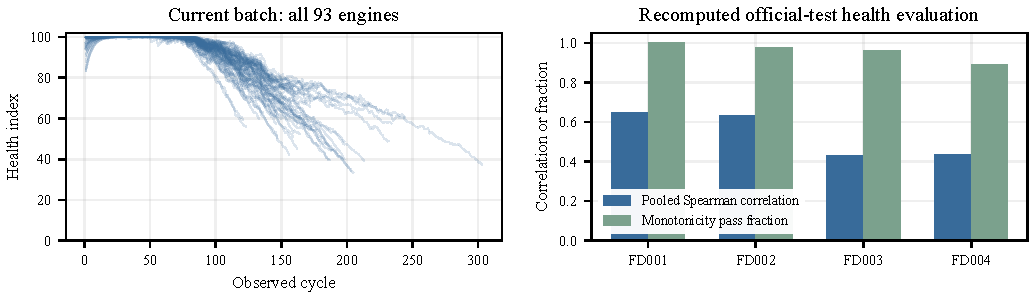
\includegraphics[width=\textwidth]{health_results.pdf}
\caption{Health evidence with populations distinguished. Left: all current-batch health trajectories, without selecting a favorable engine or adding evaluation smoothing. Right: recomputed official-test pooled rank correlation and the defined tolerance-based monotonicity fraction.}
\label{fig:health}
\end{figure*}

\subsection{Explanation and Implementation Checks}
The saved explanation evaluation covers 1,193 current-batch explanation records, rather than the entire official benchmark. Completeness and identity-consistency fractions are 1.0 under automated field and alignment checks. Local SHAP is computed for 128 records, or 10.73\% coverage, with no failed attempted rows. Maximum additive reconstruction error is $8.77\times10^{-7}$ and maximum monitoring-reference mismatch is zero. Quantitative health decomposition covers all 1,193 records. The remaining 1,065 records are not locally SHAP-explained; complete narrative fields must not be mistaken for complete attribution coverage.

Independent paper checks reproduce all 104,897 test RUL labels from the raw files and match the saved confusion counts and metrics. Reconstructing the average of the four detector scores gives a maximum fused-score difference of $3.33\times10^{-16}$. The saved activation verification also records finite detector scores and unchanged reference and health artifacts. These checks support traceability and numerical consistency, not physical diagnostic correctness.

\section{Discussion and Limitations}
The main empirical finding is a distinction between useful residual ranking, continuous health tracking, and the chosen alert policy. The system ranks the distant condition bands well, but the current equal-weight ensemble and cutoff sacrifice critical recall. The fixed linear baseline performs better on F1 and recall for these proxy labels. Thus, the evidence supports the monitoring architecture and its auditability, while providing no basis to claim that four detectors outperform simpler classification.

Any fusion-weight or threshold refinement should use development engines under a specified false-alert cost, then be evaluated on fresh trajectories withheld before that refinement. Changing the threshold to improve the official-test score would further adapt to an already reused benchmark. A controlled future study should also compare recalibrated single detectors, leave-one-detector-out fusion, context removal, and commissioning removal under the same engine roles. The present individual-score curves do not establish those causal component effects.

Several limits constrain interpretation. First, RUL bands are indirect condition labels with a large excluded intermediate band. Confirmed faults, transient disturbances, missing-data mechanisms, and onset times need separate labels. Second, historical benchmark inspection introduces adaptive evaluation bias that engine-disjoint current fitting and bootstrap intervals cannot remove. Third, the 30-cycle healthy commissioning assumption may be violated when an engine is already deteriorated or its prefix is unavailable. Fourth, gap handling differs across implementations: covariance and alert persistence reset on cycle gaps, while recurrent windows use ordered observations and health EWMA continues within an engine. The reported complete trajectories do not establish robustness to irregular or interrupted telemetry.

Finally, explanation completeness and SHAP additivity are numerical checks. They do not verify physical root causes, operator usefulness, or failure probability calibration. No expert study, prospective fleet trial, hardware-specific real-time latency study, maintenance-cost experiment, or safety benefit is demonstrated here. These remain evaluation requirements rather than inferred consequences of benchmark scores.

\section{Conclusion}
This paper presents a context-aware anomaly and health monitoring component with frozen operating references, causal commissioning, four-detector fusion, continuous health tracking, and auditable evidence. On reused C-MAPSS test trajectories, it attains ROC AUC 0.9952, F1 0.7426, critical recall 0.6321, and 181 healthy-proxy false-alert rows. It detects critical observations in 131 of 159 eligible engines, while the health index provides measurable degradation trajectories. Comparison with a stronger fixed linear proxy classifier makes the current fusion limitation explicit. The evidence supports a reproducible monitoring system and a clear experimental basis for further development; independent fault labels and previously unseen trajectories are required to establish fault-detection validity and external generalization.

\balance
\bibliographystyle{IEEEtran}
\bibliography{references}
\end{document}
